\documentclass[12pt]{article}
\usepackage{amsmath,amssymb,amsthm,amsfonts,verbatim}
\usepackage{microtype}
\usepackage{url}
\usepackage{graphicx}
\usepackage{psfrag}
\usepackage{cite}
\usepackage{subfigure}
\usepackage{stfloats}
\usepackage{float}
\usepackage{epstopdf}
\usepackage{caption}
\usepackage{booktabs}
\usepackage{hyperref}


\addtolength{\evensidemargin}{-.8in}
\addtolength{\oddsidemargin}{-.8in}
\addtolength{\textwidth}{1.4in}
\addtolength{\textheight}{1.9in}
\addtolength{\topmargin}{-.7in}

\theoremstyle{plain}
\theoremstyle{definition}
\newtheorem{theorem}{Theorem}[section]
\newtheorem{corollary}[theorem]{Corollary}
\newtheorem{proposition}[theorem]{Proposition}
\newtheorem{fact}[theorem]{Fact}
\newtheorem{lemma}[theorem]{Lemma}
\newtheorem{claim}[theorem]{Claim}
\newtheorem{conjecture}[theorem]{Conjecture}
\newtheorem{question}[theorem]{Question}
\newtheorem{definition}[theorem]{Definition}
\newtheorem{example}[theorem]{Example}
\newtheorem{exercise}[theorem]{Exercise}
\newtheorem{challenge}[theorem]{Challenge Problem}

\title{\vspace{-50pt}\textbf{EE 407\\Homework 1}\\
\large Introduction to Simulink \\ Due 23:55, 18.10.2017}
\author{}

\newcommand{\Q}{\mathbb{Q}}
\newcommand{\R}{\mathbb{R}}
\newcommand{\Z}{\mathbb{Z}}
\newcommand{\C}{\mathbb{C}}

% \DeclareMathOperator{\sin}{sin}   %% just an example (it's already defined)
\DeclareMathOperator{\norm}{norm}

\renewcommand{\baselinestretch}{1.2}
\date{}
\begin{document}
\maketitle
\setcounter{section}{0}
\vspace{-70pt}
%\normalsizesimulink


\section{Introduction}
The objective of this homework is to get you acquainted with Simulink which is one of the essential software tools that will be extensively used within this course.

Simulink is a block diagram environment for multidomain simulation and Model-Based Design. It supports simulation, automatic code generation, and continuous test and verification of embedded systems. Simulink provides a graphical editor, customizable block libraries, and solvers for modeling and simulating dynamic systems. 
It is integrated with MATLAB, enabling you to incorporate MATLAB algorithms into models and export simulation results to MATLAB for further analysis, \cite{SimulinkIntro}.

You are asked to use a MATLAB version that is not older than 2016a since this will provide some desired properties for flawless integration of other software components with Simulink in upcoming weeks.

\textbf{If you are not quite familiar with Simulink, it will be very beneficial for you to take a look at the following sources before attacking to this homework.}
\begin{itemize}
	\item A 2-minute getting started video,\\
	\url{https://www.mathworks.com/videos/getting-started-with-simulink-69027.html}	
	
	\item Step by step introduction to Simulink (estimated study time: 1.5 hour).\\
	\url{http://www.ctms.engin.umich.edu/CTMS/index.php?aux=Basics_Simulink}
\end{itemize}


\section{Questions}
	 In implementing the steps of the homework, you are expected to submit two separate Simulink models (with .slx extension) along with a report as a .pdf file. Bundle these files together and compress (as .zip) with the following name format: \textit{EE407\_eXXXXXX\_HW1}. Also note that you will submit your files via ODTUClass.
	
	\begin{enumerate}	
	\item \textbf{Mass Spring Damper System Simulation}
	You are all familiar with Mass Spring Damper (MSD) system depicted in Fig. \ref{fig:MSD}, \cite{EE302}. In a nutshell, the spring force is proportional to the displacement of the mass, $x$, and the viscous damping force is proportional to the velocity of the mass, $v=\dot{x}$. Note also that $x=0$ corresponds to the position of the mass when the spring is not stretched, and positive $x$ direction, ($\longrightarrow$), is indicated on the figure.
	
	\begin{figure}[!htb]
		\centering
		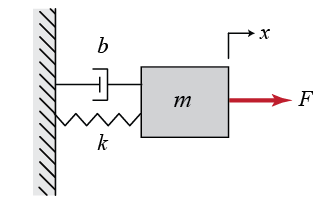
\includegraphics[width=.4\textwidth]{Figures/MassSprinDamper.png}
		\caption{}
		\centering
		\label{fig:MSD}
	\end{figure}

	\begin{enumerate}
		\item Firstly, you are to write down the state-space model of the system when the state vector is determined to comprise of position and velocity, $\mathbf{x} = \left[ \begin{array}{c} x\ \  \dot{x} \end{array}\right]^T$, the input is applied force, $F$, and the output is position, $y = \left[ \begin{array}{cc} 1 & 0 \end{array} \right] \mathbf{x}$.
		
%		$$ \mathbf{\dot{x}} = \left[ \begin{array}{c} \dot{x} \\ \ddot{x} \end{array} \right] = \left[ \begin{array}{cc} 0 & 1 \\ -\frac{k}{m} & -\frac{b}{m} \end{array} \right] \left[ \begin{array}{c} x \\ \dot{x} \end{array} \right] + \left[ \begin{array}{c} 0 \\ \frac{1}{m} \end{array} \right] F(t) $$

		\item Open a new Simulink model. Build a model of the MSD system by utilizing the built-in \textit{State-Space} block available in Simulink Library. The input of the block is to represent applied force, $F$ and the output is to be position of the mass.
		
		\item For the following subitems you will simulate the model when the applied force is a unit step function starting at t = 5 sec, i.e., $u(t-5)$. At each step, only a single parameter will be varied and corresponding system responses will be observed. Then, these responses will be investigated comparatively. You are to determine the duration of each simulation regarding to make sure that all \textit{'interesting'} observations will have been made at the end of this period.
		\textbf{In your report, include a plot exhibiting two system responses for each step.}		
		\textbf{Important:} All plots should have a title, labeled axes (with units), and reasonable axis limits.

			\begin{enumerate}
				\item Simulate the model for $(m = 1 kg,\ b = 0.2 Ns/m,\ k = 1 N/m)$ and $(m = 1 kg,\ b = 0.2 Ns/m,\ k = 0.2 N/m)$ parameter sets. Compare two output signals and command on the relation between spring constant and motion of the mass.
				\item Simulate the model for $(m = 1 kg,\ b = 0.2 Ns/m,\ k = 1 N/m)$ and $(m = 10 kg,\ b = 0.2 Ns/m,\ k = 1 N/m)$ parameter sets. Compare two output signals and command on the relation between $m$ and motion of the mass.
				\item Simulate the model for $(m = 1 kg,\ b = 0.2 Ns/m,\ k = 1 N/m)$ and $(m = 1 kg,\ b = 2 Ns/m,\ k = 1 N/m)$ parameter sets. Compare two output signals and command on the relation between viscous damping coefficient and motion of the mass.
			\end{enumerate}
				
		\item \label{stepKey} Set the parameters as $(m = 1 kg,\ b = 0.2 Ns/m,\ k = 1 N/m)$. Run the simulation for an input force whose value is equal to $1 N$ in $t = [0, 20)$ and $0 N$ elsewhere.
		To build such an input signal you are allowed to employ only \textit{Clock} and \textit{Switch} blocks. Your model should look similar to the one illustrated in Fig. \ref{fig:Clock}. \textbf{Insert the plot demonstrating the output signal into your report.} \textbf{You are asked to submit this final version of the Simulink model for Question 1.}
		
		\begin{figure}[!htb]
			\centering
			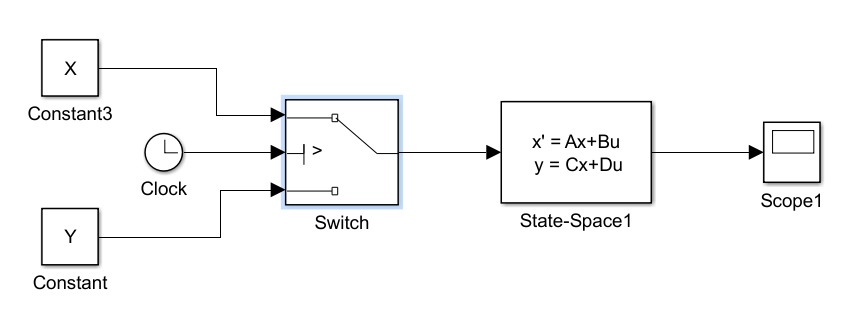
\includegraphics[width=.7\textwidth]{Figures/ClockSwitchUsage.png}
			\caption{}
			\centering
			\label{fig:Clock}
		\end{figure}
	
		\item In this step you are to evaluate time resolution of the output signals observed in \textit{d}. Observe time differences between successive data points, $\delta t$, in the output signal. Does $\delta t$ change during simulation? If Yes, what might be the reason for Simulink to simulate the model in such a fashion? What might be possible advantages/ disadvantages of this technique?
		
		\item Open \textit{Model Configuration Parameters} of the model. Under \textit{Solver} tab, choose \textit{Fixed Step} option and set sampling time as 0.01 sec. Run the simulation again. Comment on the effect of change in the solver.

	\end{enumerate}
	

	\item \textbf{Propeller Levitated Arm Simulation}
	
	In this section, you are going to simulate a Propeller Levitated Arm (PLA) with which you have already been introduced via bonus project of EE302. The system is illustrated in Fig. \ref{fig:PLA}. 
	
	\begin{figure}[!htb]
		\centering
		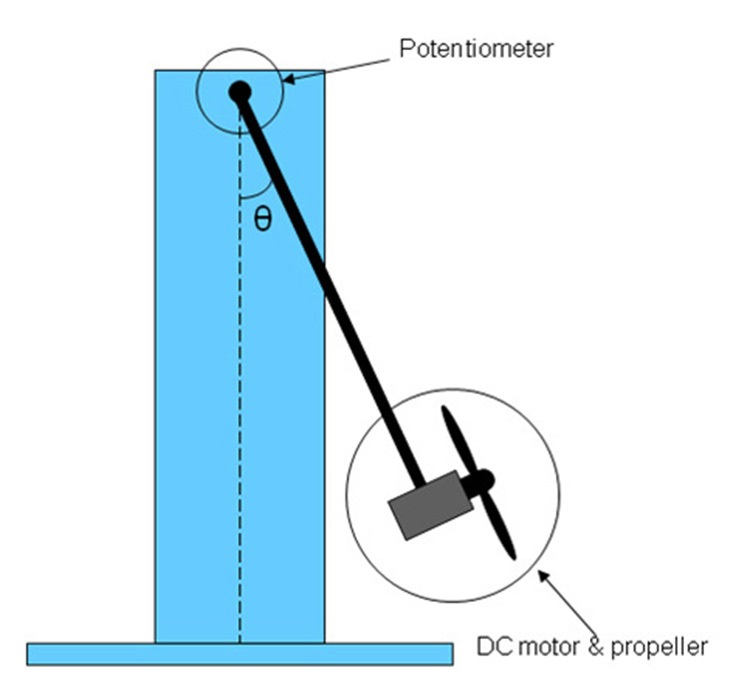
\includegraphics[width=.3\textwidth]{Figures/PropellerLevitatedArm.jpg}
		\caption{}
		\centering
		\label{fig:PLA}
	\end{figure}
	
	The differential equation describing the dynamic behavior of the system is as given:	
	\begin{equation} \label{eq:PropEq}
	m L^2 \ddot{\theta} = -c\dot{\theta} - m g L sin(\theta) + u
	\end{equation}	
	where $\theta$ is angular position of the arm, $m$ is the total mass of the propeller and DC motor, $L$ is length of the arm, $c$ is viscous damping coefficient, $g$ is gravitational acceleration and $u$ is thrust produced by the propeller. (Note that the arm is assumed to be massless.)
	
	\begin{enumerate}
		\item Open a new Simulink model. Create a subsystem, \cite{SimulinkSubsystem}, whose input is thrust force and output is angular position. \underline{Do NOT} linearize the dynamics of the system given in \eqref{eq:PropEq}. 
		\textbf{Submit this model for Question 2.}
		
		\textbf{Hint: A partially constructed model of the PLA where some blocks are not shown is demonstrated in Fig. \ref{fig:PropSim}.}
		
		\item  What do X, Y and Z signals in Fig. \ref{fig:PropSim} stand for in the real system?

		\begin{figure}[!htb]
			\centering
			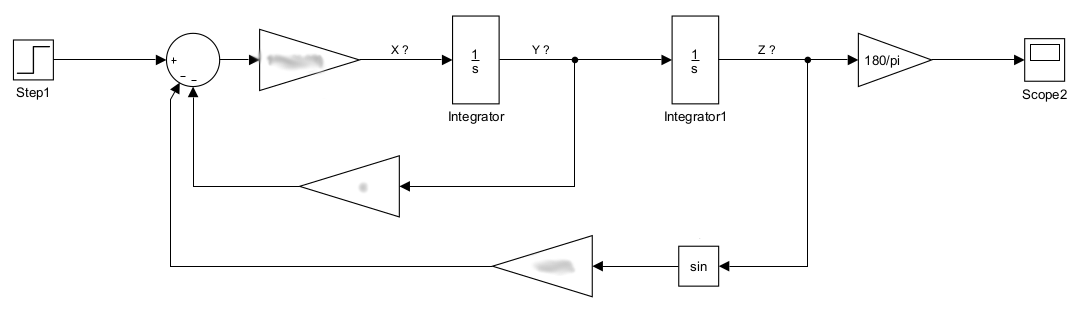
\includegraphics[width=1\textwidth]{Figures/PropellerSimModel.png}
			\caption{}
			\centering
			\label{fig:PropSim}
		\end{figure}
			
		\item Is this model valid for all values of the state vector? Or is there a range of $\theta$ for the model to be consistent with real dynamics of the system?							
		
		\item Set $m = 1\ kg,\ L = 2\ m,\ g = 9.81\ m/s^2,\ c = 0.5\ kgm^2/s$, then run two separate simulations one for an input force of $14 Nm$ and the other for $15 Nm$. \textbf{Record the angular position of the arm in degrees and put them into your report.} Why is a slight difference in the thrust resulted in such a drastic change in the response of the system? 

	\end{enumerate}
		
\end{enumerate}

\pagebreak
\bibliographystyle{IEEEtran}

\bibliography{research}

\end{document}